%%
%% This is file `tikzposter-template.tex',
%% generated with the docstrip utility.
%%
%% The original source files were:
%%
%% tikzposter.dtx  (with options: `tikzposter-template.tex')
%%
%% This is a generated file.
%%
%% Copyright (C) 2014 by Pascal Richter, Elena Botoeva, Richard Barnard, and 
%%Dirk Surmann
%%
%% This file may be distributed and/or modified under the
%% conditions of the LaTeX Project Public License, either
%% version 2.0 of this license or (at your option) any later
%% version. The latest version of this license is in:
%%
%% http://www.latex-project.org/lppl.txt
%%
%% and version 2.0 or later is part of all distributions of
%% LaTeX version 2013/12/01 or later.
%%


\documentclass{tikzposter} %Options for format can be included here

\usepackage{showframe}
\usepackage{todonotes}
\usepackage[ruled]{algorithm2e}
\usepackage[tikz]{bclogo}
\usepackage{lipsum}
\usepackage{amsmath}
\usepackage{algorithm}
\usepackage{algorithmic}
\usepackage{booktabs}
\usepackage{longtable}
\usepackage[absolute]{textpos}
\usepackage[it]{subfigure}
\usepackage{graphicx}
\usepackage{cmbright}
%\usepackage[default]{cantarell}
%\usepackage{avant}
%\usepackage[math]{iwona}
\usepackage[math]{kurier}
\usepackage[T1]{fontenc}


%% add your packages here
\usepackage{hyperref}
% for random text
\usepackage{lipsum}
\usepackage[english]{babel}
\usepackage[pangram]{blindtext}
\colorlet{backgroundcolor}{blue!10}

% Title, Author, Institute
\title{Flip 00 project final report}
\author{Rongxin Xu}
\institute{ Hunan University, China
}

\usetheme{Wave}


\begin{document}
	
	
	\colorlet{blocktitlebgcolor}{blue!23}
	
	% Title block with title, author, logo, etc.
	\maketitle
	
	\begin{columns}
		% FIRST column
		\column{0.5}% Width set relative to text width
		
		
		\block{Introduction}{
			This is a problem with time-series prediction.
			After a month of making scientific observations 
			and taking careful measurements, 
			can predict total sales for every product and store in the next 
			month.
			The raw dataset contains train set with 2935849 
			samples and 214200 unlabeled samples as test set.
			Through the train data, predict total sales for every product and 
			store in 
			the next month.
			\vspace{.5cm}
			\begin{description}
				\item[id]  an Id that represents a (Shop, Item) tuple within 
				the test set.
				\item[shop\_id] unique identifier of a shop.
				\item[item\_id] unique identifier of a product.
				\item[item\_category\_id] unique identifier of item category.
				\item[item\_cnt\_day] percentage of soul in the creature.
				\item[item\_price] current price of an item.
				\item[date] date in format dd/mm/yyyy.
				\item[date\_block\_num] unique identifier of item category.
				\item[item\_name] name of item.
				\item[shop\_name] name of shop.
				\item[item\_category\_name] name of item category.
			\end{description}
			\vspace{.3cm}
		}
		
		\block{Data Visualization}{
			The Histogram 
			shows the distribution of the various attributes. It seems that 
			item\_id and 
			shop\_id has a huge impact on sales and sales tend to decline with 
			the date.
			Through the Boxplot, 
			we know that the outliers are very small,
			so can be ignored.
			\vspace{.5cm}
			\begin{center}
				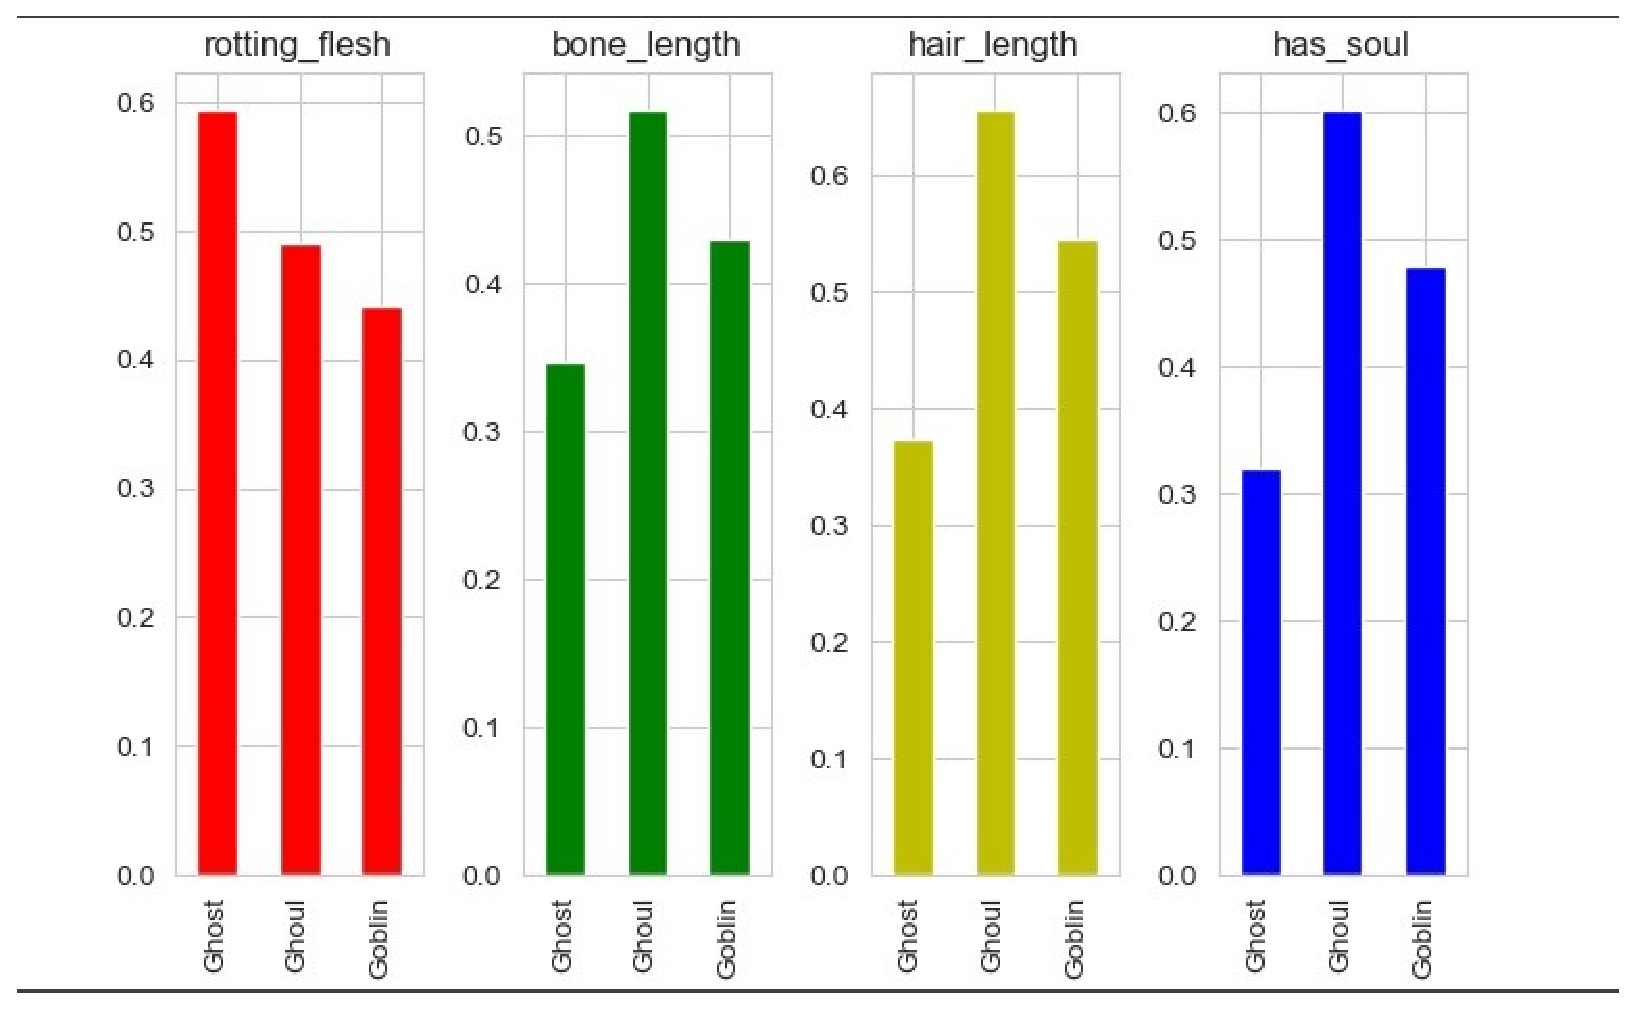
\includegraphics[width=.3\linewidth]{figures/his_1.eps}
				\quad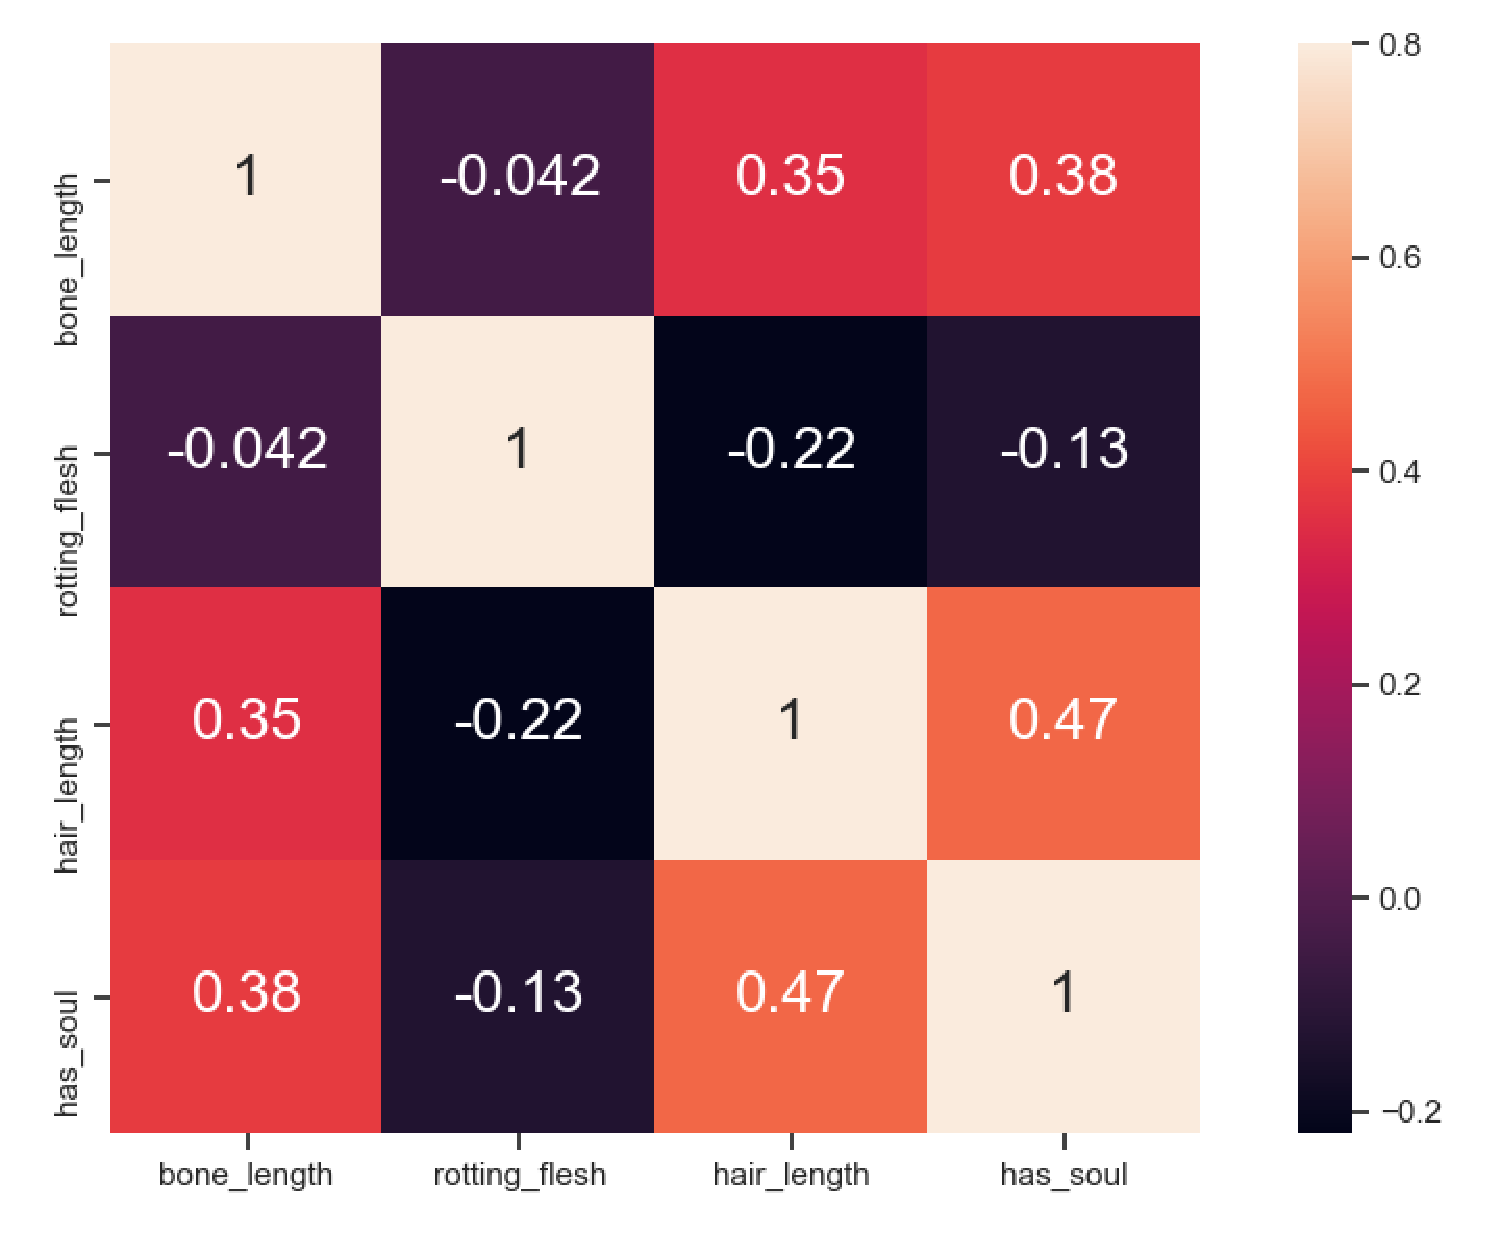
\includegraphics[width=.3\linewidth]{figures/corr.eps}
				\quad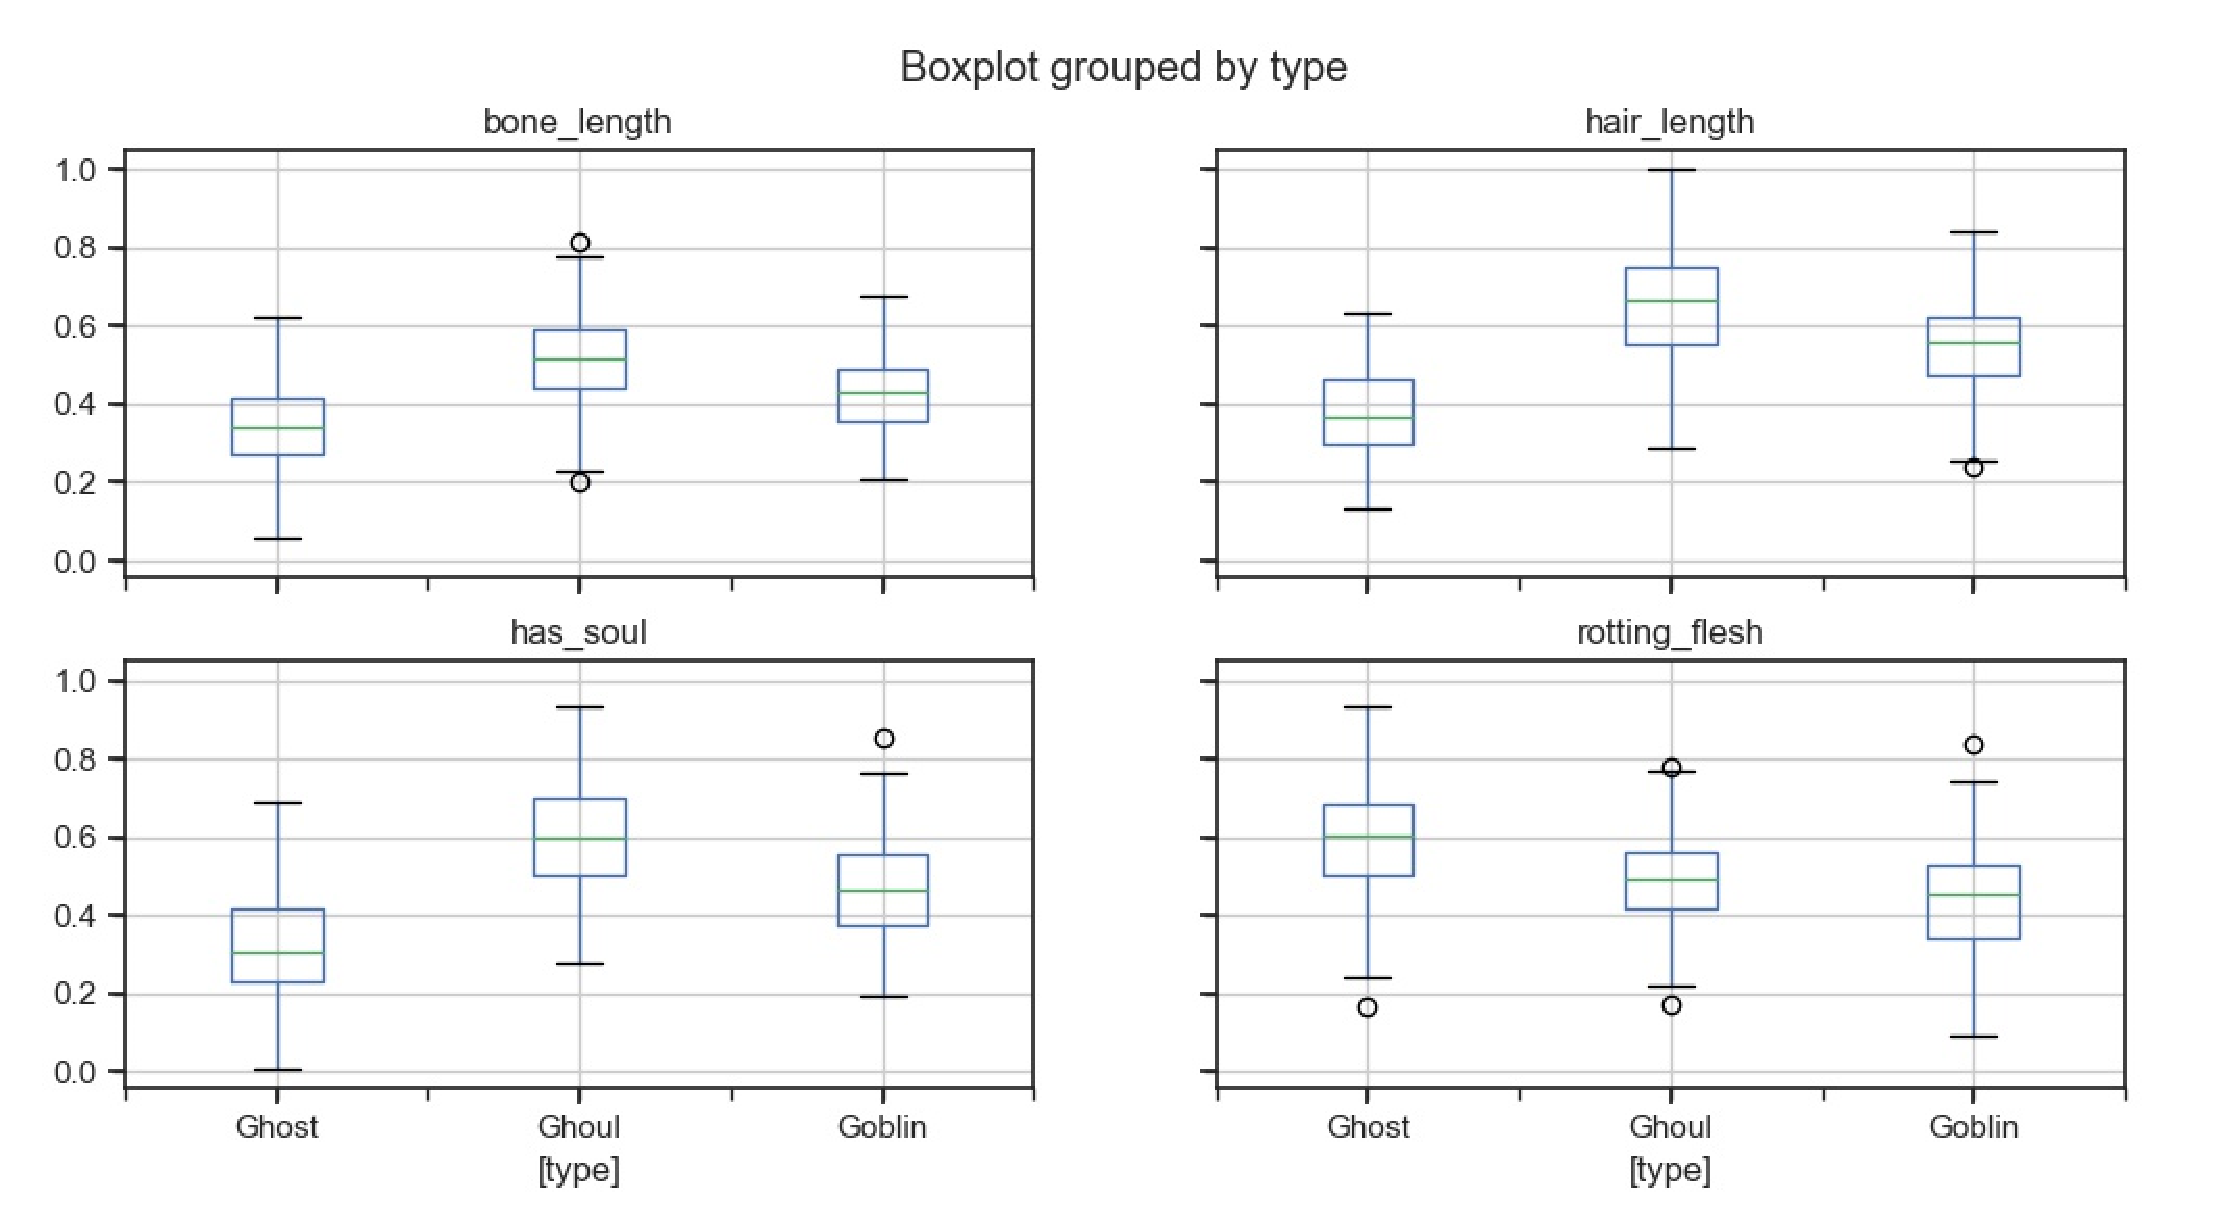
\includegraphics[width=.3\linewidth,height=.25\linewidth]{figures/boxplot.eps}
					
			\end{center}
			\vspace{.3cm}
		}
		
		\block{Feature Engineering}{
			
			\vspace{.5cm}
			Using the Feature Importance 
			this function of Random Forest
			to select the most important features
			to form a new train data. I take these 
			features to form a new train datad.
			\vspace{.5cm}
			\begin{center}
				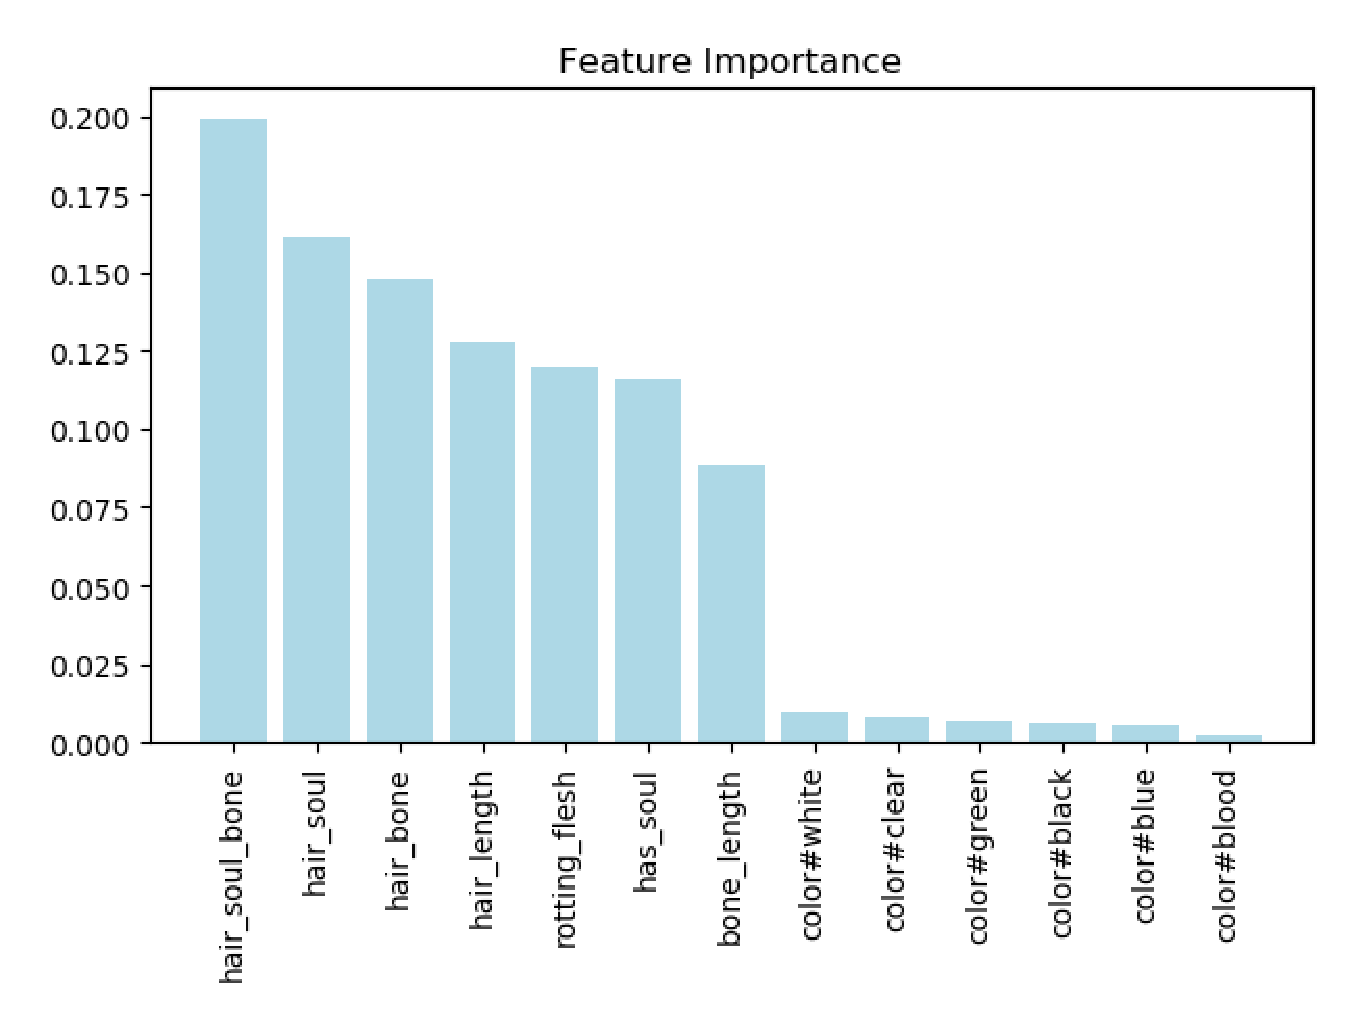
\includegraphics[width=.3\linewidth]{figures/FEATURE.eps}
			\end{center}
		}
		
		
		
		
		\column{0.5}
		
		\block{Algorithm}{
			To combine the base models as 1st level 
			model predictions, I'll use a simple 
			linear regression. As I'm only feeding 
			the model with predictions 
			I don't need a complex model.
			\vspace{.5cm}
			\begin{itemize}
				\item Base Models
				\
				\begin{itemize}
					\item RandomForest
					\item XGBoost
					\item LSTM
					\item Linear regression
					\item KNN
				\end{itemize}
				\item Ensemble Model
				\
				\begin{itemize}
					\item Linear regression
				\end{itemize}
			\end{itemize}
			\vspace{.5cm}
		}
		
		
		\block[titleleft]{Experiment Result}
		{
			The tables below shows that the rmse of 
			each model, RandomForest and XGBoost 
			perform better, and there is not much 
			difference between the other models.
			\vspace{.4cm}
			\begin{itemize}
				\item Forecast Result of Base Models
			\end{itemize}
			\vspace{.5cm}
			\begin{center}
				\begin{tabular}{ccccccc}
					%\bottomrule
					\toprule
					& RandomForest & XGBoost & LSTM & Linear regression & KNN\\
					\midrule
					Train rmse & 0.8358 & 0.8327 & 0.9276 & 0.8572 & 0.6976\\
					Validation rmse & 0.8810 & 0.8959 & 0.6611 & 0.8806 & 
					0.8946\\
					\bottomrule
				\end{tabular}
			\end{center}
			\vspace{.5cm}
			The train rmse of Ensemble model is 0.764973649571408.
			
		}
		
		\block[titlewidthscale=1, bodywidthscale=1]
		{Conclusion}
		{
			\begin{description}
				\item Exploratory data analysis is 
				very important for the competition,
				Discover the imperfections of the 
				data and have a certain understanding 
				of the overall appearance of the data, 
				which will help later modeling and analysis. 
				\vspace{.5cm}
				\item The data that we have,
				needed processed in many cases.
				Data preprocessing includes 
				deal with missing data and outliers, 
				We must think carefully about the outliers, 
				such as ignoring them.
				\vspace{.5cm}
				\item The most important thing is
				feature engineering.
				We have to think carefully and 
				deal with outliers, such as ignoring 
				or deleting them.
				\vspace{.5cm}
				\item There is no best model, 
				only the best model. We should 
				try as many models as possible to 
				get the best prediction results. 
				\vspace{.5cm}
				\item Feature engineering is very 
				important and even plays a decisive 
				role in this competition.
				\vspace{.5cm}
				\item The Ensemble model may perform better 
				than a single model when dealing 
				with some complex problems.	
				\vspace{.5cm}
			\end{description}
		}
		
		
		\colorlet{notebgcolor}{blue!20}
		\colorlet{notefrcolor}{blue!20}
		\note[targetoffsetx=8cm, targetoffsety=-12cm, angle=30, rotate=15,
		radius=2cm, width=.26\textwidth]{
			Acknowledgement
			\begin{itemize}
				\item
				Thanks!
			\end{itemize}
		}
		
		
	\end{columns}
	
	\colorlet{notebgcolor}{blue!20}
	\colorlet{notefrcolor}{blue!20}
	\note[targetoffsetx=-13cm, 
	targetoffsety=-20cm,rotate=0,angle=180,radius=8cm,width=.96\textwidth,innersep=.4cm]
	{
		\begin{minipage}{0.3\linewidth}
			\centering
			\includegraphics[width=24cm]{logos/tulip-wordmark.eps}
		\end{minipage}
		\begin{minipage}{0.7\linewidth}
			{ \centering
				Flip 00 project final report,
				29/11/2019, changsha, China
			}
		\end{minipage}
	}
	
\end{document}

